\begin{quote}
    \textit{``There are no dumb questions, there can only be dumb answers.''}
    
    ---Nemanja Kaloper
\end{quote}

\begin{exm}
    Let us try to evaluate
    \begin{equation}
        \int_0^\infty dx \frac{x^p}{1+x^2}, \quad 0 < p < 1.
    \end{equation}
    The integrand has a branch point at $x=0$, so we can choose an contour to perform the integral. The value of the contour integral is
    \begin{equation}
        \oint = I + \int_{C_R} - e^{2\pi i p} I +\int_{C_\rho},
    \end{equation}
    where $C_R$ indicates the circle at infinity and $C_\rho$ indicates the small semicircle about the origin. The $C_R$ integral is zero since this integral goes as $R^{p-1}$ as $R\to \infty$, while the $c_\rho$ integral is zero since this goes as $\rho^{p+1}$ as $\rho\to 0$.
    
    Thus
    \begin{equation}
        \oint = (1-e^{2\pi i p})I
    \end{equation}
    and by the residue theorem, the contour integral is
    \begin{equation}
        \oint = 2\pi i \bkt{\frac{i^p}{2i} + \frac{(-i)^p}{-2i}}.
    \end{equation}
    Solving, we find that
    \begin{equation}
        I = \frac{\pi}{2\cos \paren{\frac{p\pi}{2}}}.
    \end{equation}
    Notice this integral has singularities at odd integer $p$. This is very similar to the gamma function, which has an integral representation $\Gamma(x) = \int_0^\infty dt \, t^{x-1}e^{-t}$ and diverges for negative integer $x$.
\end{exm}

We can use branch cuts to compute certain integrals. We previously computed
\begin{equation}
    \int_0^\infty dx \frac{1}{x^3+1}
\end{equation}
and also
\begin{equation}
    \int_0^\infty dx \frac{\ln x}{1+x^3}
\end{equation}
over a very similar contour.
\begin{exm}
    Let us now show that we can use the second integral with the branch cut to work out the first one. That is, we shall choose the contour
    \begin{center}
    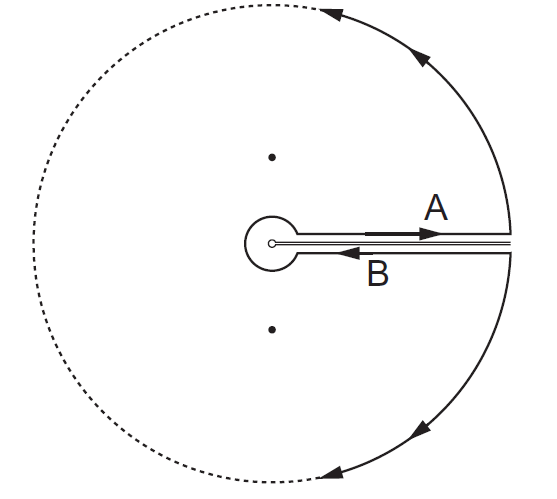
\includegraphics{2020/02/20200224_contour.PNG}
    \end{center}
    and see what this does for us.
    
    Note the poles marked here are for the previous example. Here, we have poles at $e^{\pi i/3},e^{\pi i}, e^{5\pi i /3}$ and we will need to evaluate the three residues. Now as before we get the integral over the upper segment $A$ and the lower segment $B$; $\ln x dx$ goes to zero quickly about the small circular region near the origin, and this integral goes away as $\ln x/x^2$ as $x\to \infty$. Hence our integral is
    \begin{equation}
        \oint = \int_0^\infty dx \frac{\ln x}{1+x^3} - \int_0^\infty dx \frac{\ln x +2\pi i}{1+x^3} = -2\pi i I,
    \end{equation}
    where $I$ is the integral we wanted. Since the contour integral is $2\pi i\times{}$ the residues, we find that
    \begin{equation}
        -I= \text{Res}_1 + \text{Res}_2 + \text{Res}_3.
    \end{equation}
    If we work it out, we find that
    \begin{equation}
        I= \frac{2\pi}{3\sqrt{3}},
    \end{equation}
    just as before.
\end{exm}
%It is a coincidence, but it is not an accidental coincidence.
%There are no dumb questions, there can only be dumb answers.

\begin{exm}
    Consider
    \begin{equation}
        \int_0^\infty dx \frac{x}{\sinh x}.
    \end{equation}
    The integrand is even, so we can extend it as
    \begin{equation}
        \frac{1}{2}\Int dx \frac{x}{\sinh x}.
    \end{equation}
    As $|x|$ grows large, the exponentials force this to converge. But how should we close the contour? The Jordan lemma doesn't apply. However, notice the following.
    \begin{equation}
        \sinh iy = \frac{1}{2} (e^{iy} -e^{-iy}) = i \sin y.
    \end{equation}
    Recall that $\sinh(x)$ follows the addition formula
    \begin{equation}
        \sinh(x+i\pi) = \sinh x \cosh (i\pi) + \cosh x \sinh (i\pi),
    \end{equation}
    so because $\sinh i\pi=i\sin \pi =0$ and $\cosh i\pi = \cos \pi =-1$, we find that
    \begin{equation}
        \sinh(x+i\pi) =-\sinh x.
    \end{equation}
    We see that $\sinh$ is $2\pi$-periodic in the imaginary direction. Therefore this suggests that we take a rectangular contour of height $i\pi$ and length $2L$. The sides are
    \begin{equation}
        \int_0^\pi i dy \frac{\pm L + iy}{\sinh(\pm L +iy)},
    \end{equation}
    which goes away as $L\to \infty$, so our integral is
    \begin{equation}
        \oint = \Int + \Int dx \frac{x +i\pi}{\sinh x}.
    \end{equation}
    If we treat the $\frac{i\pi}{\sinh x}$ as a principal value, we find that its principal value is zero. Hence
    \begin{equation}
        \oint =2\Int dx \frac{x}{\sinh x},
    \end{equation}
    and all we need to do is add the residues. This has a pole at $z=\pi i$, so when we take the residue we find that it is
    \begin{equation}
        \lim_{z\to \pi i} (z-\pi i) \frac{z}{\sinh z} =-\pi i
    \end{equation}
    and so
    \begin{equation}
        I= \frac{\pi^2}{4}.
    \end{equation}
\end{exm}